\section{Supplementary material}

\subsection{Agreement of the grid and the paired runs}
The full grid and the paired W3/G128 exports were produced by separate evaluation runs of the same checkpoints.
On the \V{consistContexts} contexts present in both, baseline top-1 differs by at most \V{consistFp} points and W3/G128 top-1 by at most \V{consistQ} points.

\subsection{Matching bin width}
With bin widths 0.025, 0.05 and 0.1, the reduction of the retention gap ranges from \V{reductionMinAll}\% to \V{reductionMaxAll}\% over the nine settings.

\subsection{W3/G128 diagnostics}
\Cref{tab:diagnostics} lists the final-layer CKA, the class-offset correction and the competitor comparison of each setting.

\begin{table}[h]
\centering
\caption{W3/G128 diagnostics over the {\V{nDatasets}} datasets. CKA: median final-layer CKA. Offset: mean top-1 change in points after the cross-fitted class-offset correction, beside the mean of five shuffled-class controls. $\Delta$Brier ($\times 10^{3}$): change in damage Brier score from adding competitor counts.}
\label{tab:diagnostics}
\setlength{\tabcolsep}{3pt}
\small
\begin{tabular}{llrrrr}
\toprule
Backbone & Strategy & CKA $\uparrow$ & Offset & Shuffled & $\Delta$Brier $\downarrow$ \\
\midrule
ViT-B/16 & FT & 0.88 & 0.64 & $-$0.94 & 3.71 \\
ViT-B/16 & FZ & 0.91 & 1.52 & $-$1.55 & $-$4.58 \\
ViT-B/16 & CAL & 0.95 & 1.29 & $-$1.13 & $-$6.07 \\
Swin-B & FT & 0.87 & 1.91 & $-$1.47 & $-$2.34 \\
Swin-B & FZ & 0.91 & 4.15 & $-$2.34 & $-$9.32 \\
Swin-B & CAL & 0.90 & 2.47 & $-$1.60 & $-$2.22 \\
BEiTv2-B & FT & 0.78 & 2.78 & $-$0.93 & 0.01 \\
BEiTv2-B & FZ & 0.16 & 2.06 & $-$1.19 & $-$0.19 \\
BEiTv2-B & CAL & 0.86 & 11.31 & $-$7.72 & $-$2.39 \\
\bottomrule
\end{tabular}
\end{table}


\subsection{Correlates of the difficulty score}
\Cref{tab:properties} lists the Spearman correlation of every measured property with the \term{difficulty score}.

\begin{table}[h]
\centering
\caption{Spearman correlation of each property with the difficulty score over the {\V{gridDatasets}} datasets. FP: baseline top-1. Sep.: separability. H: H-score. Norm: feature norm ratio P99/P50. All are measured on the baseline except the final-layer CKA between baseline and W3/G128 features.}
\label{tab:properties}
\setlength{\tabcolsep}{1.5pt}
\footnotesize
\begin{tabular}{llrrrrrrr}
\toprule
Backbone & Strategy & $q_{10}$ & FP & $C$ & Sep. & H & Norm & CKA \\
\midrule
ViT-B/16 & FT & $-$0.96 & $-$0.97 & 0.47 & $-$0.83 & $-$0.32 & 0.42 & $-$0.20 \\
ViT-B/16 & FZ & $-$0.93 & $-$0.91 & 0.30 & $-$0.83 & $-$0.25 & $-$0.90 & $-$0.48 \\
ViT-B/16 & CAL & $-$0.82 & $-$0.84 & 0.47 & 0.11 & 0.06 & 0.48 & $-$0.03 \\
Swin-B & FT & $-$0.87 & $-$0.82 & 0.48 & $-$0.73 & $-$0.56 & $-$0.39 & $-$0.51 \\
Swin-B & FZ & $-$0.97 & $-$0.98 & 0.36 & $-$0.80 & $-$0.15 & $-$0.81 & $-$0.31 \\
Swin-B & CAL & $-$0.65 & $-$0.67 & 0.49 & 0.10 & $-$0.43 & $-$0.10 & $-$0.19 \\
BEiTv2-B & FT & $-$0.53 & $-$0.45 & 0.03 & $-$0.44 & $-$0.27 & $-$0.19 & $-$0.35 \\
BEiTv2-B & FZ & $-$0.93 & $-$0.96 & 0.31 & $-$0.86 & $-$0.42 & 0.69 & $-$0.17 \\
BEiTv2-B & CAL & $-$0.80 & $-$0.72 & 0.21 & 0.27 & $-$0.09 & $-$0.04 & 0.25 \\
\bottomrule
\end{tabular}
\end{table}


\subsection{Local structure of the features}
\Cref{fig:tsne} shows a joint t-SNE~\cite{vandermaaten2008tsne} of baseline and W3/G128 final features for one context.
In this context, the clusters of the selected classes remain separate after quantization.

\begin{figure}[h]
  \centering
  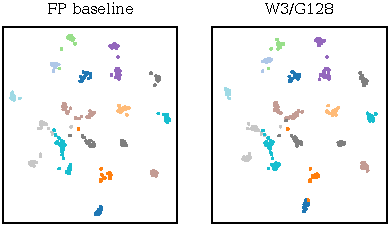
\includegraphics[width=\linewidth]{figures/tsne_cub_vit_ft.pdf}
  \caption{Joint t-SNE of the final features of ViT-B/16 FT on CUB, for \V{tsneClasses} of its \V{cubClasses} classes and all their test images, before and after W3/G128 quantization. Colors are classes.}
  \label{fig:tsne}
\end{figure}

\subsection{Swap rate by margin}
\Cref{fig:decile} relates the swap rate to the baseline margin of each image \TBD{per-image quantized predictions are needed for this figure}.

\begin{figure}[h]
  \centering
  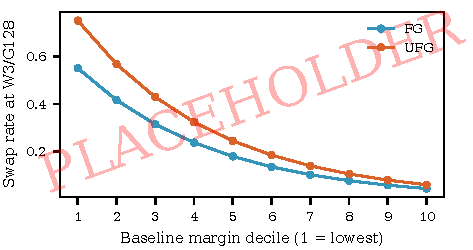
\includegraphics[width=\linewidth]{figures/swap_by_decile_placeholder.pdf}
  \caption{[PLACEHOLDER: synthetic values] Swap rate at W3/G128 by baseline margin decile within each dataset, averaged over datasets with equal weight.}
  \label{fig:decile}
\end{figure}
